\documentclass[listings]{labreport}
\subject{Компьютерная графика}
\titleparts{Лабораторная работа №2}{Использование бибилиотеки OpenGL}
\students{Лабушев Тимофей}

\usepackage{enumitem}

\begin{document}

\maketitlepage

\section*{Задание}

Средствами библиотеки OpenGL реализовать сцену, содержащую несколько типов источников
света. В центр сцены поставить примитивы (например, кубы) и объекты, выгруженные из 3D редактора,
наложить на них текстуры. Добавить перемещение камеры и динамику (движение некоторых объектов).

\section*{Описание реализации}

Сцена, созданная в 3D редакторе, экспортируется в формат FBX и считывается
программой средствами библиотеки \textit{Open Asset Import Library}. В описание сцены
входят объекты, текстуры, анимации.

Отрисовка и обработка ввода осуществляется в цикле событий, на каждой итерации которого
выполняются следующие действия:
\begin{enumerate}
  \item Переход к следующему кадру, если воспроизводится анимация.
    \vspace*{0.2em}

    {\small Поддерживается лишь простая анимация, в которой каждый кадр представляет собой новую матрицу модели.}

  \item Создание карты теней для каждого источника освещения.
    \vspace*{0.2em}

    {\small В текстуру глубины сохраняется расстояние от источника до каждого объекта на сцене.}

  \item Отрисовка каждого объекта на сцене.
    \vspace*{0.2em}

    {\small Вершинному шейдеру передается матрица модели текущего объекта, на основе которой вычисляются мировые координаты, и матрицы вида и проекций камеры, которые определяют положение объекта от лица пользователя.}

    \vspace*{0.2em}

    {\small Фрагментный шейдер задает цвет пикселя на основании текстуры объекта и освещения. Для расчетов освещения используется простая модель, в которой цвет рассеивания прибавляется пропорционально
    увеличению угла между поверхностью и направлением светa. Результирующий цвет умножается на коэффициент, обратный тени. Тень определяется сэпмлированием карты теней с помощью \texttt{sampler2DShadow},
    возвращаемое значение которого — результат сравнения Z-координаты текущего объекта c глубиной объекта, освещаемого источником в этой точке.}

    \vspace*{0.2em}

    {\small На сцене присутствует два источника освещения: направленный (лунный свет) и прожектор (экран компьютера). Последний отличается затуханием по мере увеличения расстояния до объекта и отсечкой света за пределами заданного конуса.}

  \item Обработка пользовательского ввода.

    {\small Перед перемещением камеры выполняется проверка на наличие коллизии между объектом игрока и каким-либо предметом на сцене. Для этого каждый объект ограничивается произвольно ориентированной областью
    в виде прямоугольного параллелепипеда (\textit{oriented bounding box}).}
  
    {\small Считывание положения мыши и ввода с клавиатуры осуществляется средствами библиотеки \textit{GLFW}.}
\end{enumerate}

\section*{Скриншоты реализации}

\begin{figure}[h!]
\centering
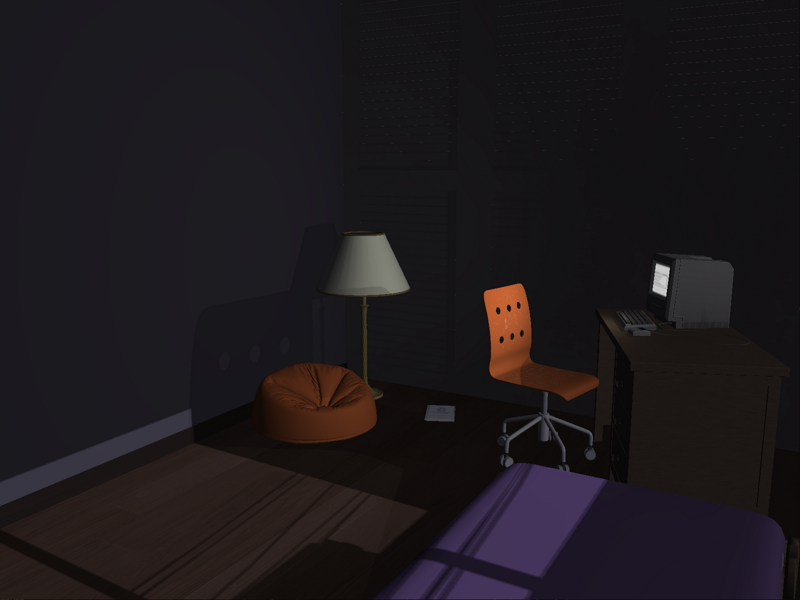
\includegraphics[width=0.8\textwidth]{screenshots/scene.png}
\caption{Вид с основной камеры на центр сцены}
\end{figure}

\begin{figure}[h!]
\centering
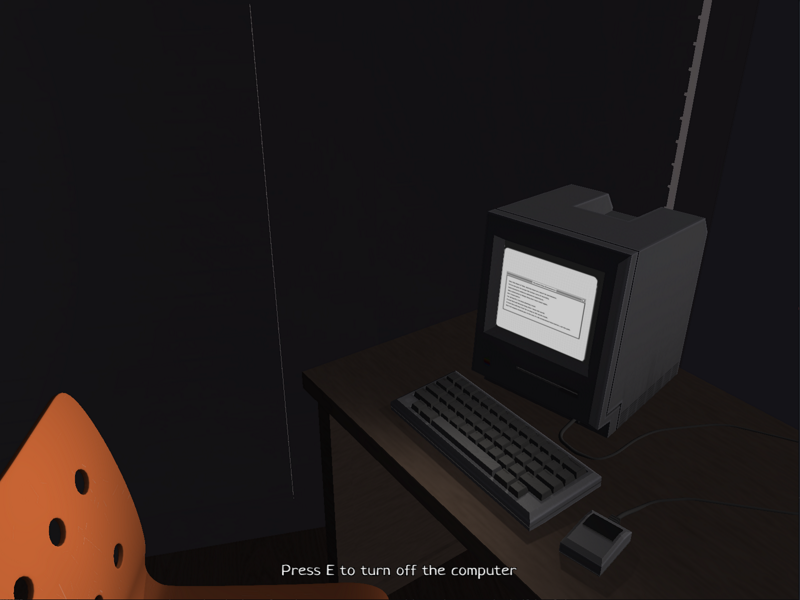
\includegraphics[width=0.8\textwidth]{screenshots/computer-interaction-on.png}
\caption{Взаимодействие с источником освещения}
\end{figure}

\begin{figure}[h!]
\centering
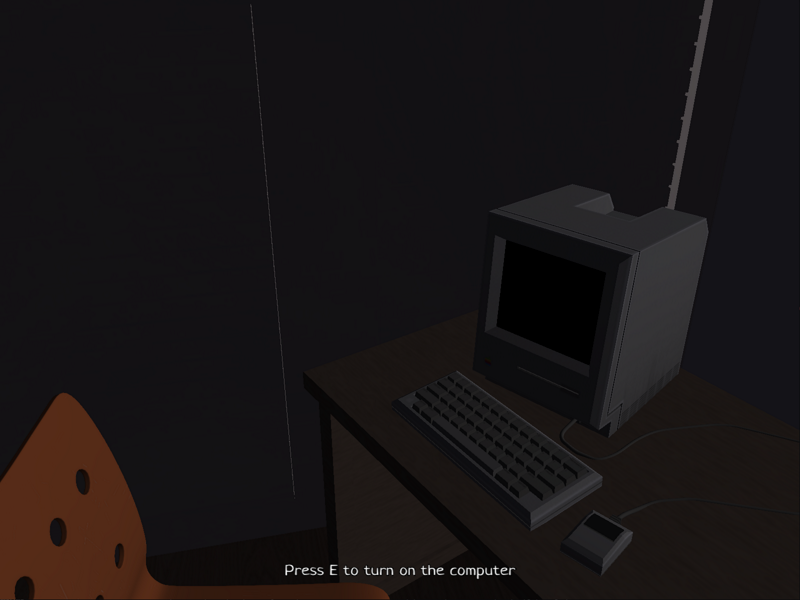
\includegraphics[width=0.8\textwidth]{screenshots/computer-interaction-off.png}
\caption{Результат взаимодействия с источником освещения}
\end{figure}

\newpage
\section*{Исходный код}

Исходный код лабораторной работы доступен по адресу:

\verb|https://github.com/timlathy/itmo-fourth-year/tree/master/Computer-Graphics-7th-Term/Lab2|.

\end{document}
